%!TEX root = ../thesis.tex

\chapter[a retrospective study on machine learning-assisted stroke recognition for medical helpline calls]{A Retrospective Study on Machine Learning-Assisted Stroke Recognition for Medical Helpline Calls}
\label{chp:paper-retrospective}
\ifthenelse{\equal{\skippapers}{true}}{}{


% cite21 = borgholt_endtoend_2020
% cite23 = hochreiter_long_1997
% cite24 = graves_connectionist_2006
% cite25 = hansen_neural_1990
% cite26 = rosenblatt_perceptron_1958
% cite27 = dwass_modified_1957
% cite28 = eden_validity_1933


\section*{Abstract}
\paragraph{Background:} Effective stroke treatment depends on recognition by call-takers at prehospital telehealth services. This study aimed to develop and assess the potential of machine learning in improving prehospital stroke recognition during medical helpline calls.
\paragraph{Methods:} We used calls from 1 January 2015 to 31 December 2020 in Copenhagen to develop a machine learning-based classification pipeline. Calls from 2021 were used for testing. Calls were transcribed using an automatic speech recognition model and then categorized as stroke or non-stroke using a text classification model.
\paragraph{Findings:} Call-takers achieved a sensitivity of 52.7\% (95\% confidence interval 49.2-56.4\%) with a positive predictive value (PPV) of 17.1\% (15.5-18.6\%). The machine learning framework performed significantly better (p < 0.0001) with a sensitivity of 63.0\% (62.0-64.1\%) and a PPV of 24.9\% (24.3-25.5\%).
\paragraph{Interpretation:} A machine learning framework for recognizing stroke in prehospital medical helpline calls may become a supportive tool for call-takers, aiding in early and accurate stroke recognition.


\section{Introduction}
Stroke is a leading cause of disability and death worldwide \cite{cite1,cite2,cite3}. Effective treatment is time-sensitive, and an optimal outcome is more likely when treatment is administered within the first four and a half hours from stroke onset \cite{cite4,cite5}. The gateway to ambulance transport and hospital admittance is through prehospital telehealth services, including emergency medical call centres, nurse advice call lines, and out-of-hours health services. In the pre-hospital setting, the use of mobile stroke units has made it possible to deliver advanced treatment faster. As the mobile stroke unit is only dispatched to patients with a suspected stroke, the impact of mobile stroke units is directly influenced by accurate call-taker recognition of stroke \cite{cite6,cite7}. Call-takers who can rapidly and accurately recognize stroke are therefore crucial in facilitating prompt care in both pre-hospital and in-hospital settings.

Despite initiatives to improve stroke recognition \cite{cite8,cite9}, approximately half of all patients with stroke do not receive the correct triage for their condition from call-takers \cite{cite10,cite11,cite12}. Most initiatives aim to improve stroke recognition by call-takers via introducing more specific assessment tools \cite{cite8,cite9} or providing specialized training \cite{cite13}. Recent advances in machine learning technology might be applied to improve stroke recognition without requiring changes to the triaging approach, and machine learning aided identification of stroke has been suggested as a means of improving mobile stroke unit effectiveness \cite{cite7}. Real-time feedback from a machine learning model can improve the recognition of out-of-hospital cardiac arrest \cite{cite14,cite15}. Therefore, this study aimed to develop and assess the potential of machine learning in improving prehospital stroke recognition during medical helpline calls.


\section{Results}

\subsection{Main results}

The classification model outperformed the call-takers (\cref{tab_retrospective:table1}), with significant differences in all metrics (p < 0.0001). Excluding the 1-1-2 call line training data significantly degraded the model's performance (p < 0.0001), despite the domain mismatch with the MH-1813 call line test data. The performance on the 2021 calls without a diagnostic category was significantly worse than that of the test set regarding F1 score, sensitivity, FPR, and FOR (p < 0.0001).

The ROC curve (\cref{fig_retrospective:figure1}, left) illustrates the potential to increase the sensitivity while maintaining a FPR lower than or equal to that of the call-takers. Similarly, the PPV sensitivity curve (\cref{fig_retrospective:figure1}, right) demonstrates that sensitivity can be improved while retaining a PPV higher than that of the call-takers. The framework can thus be tuned to a sensitivity of around 73\%, while still having a higher positive predictive value than the human call-taker (\cref{fig_retrospective:figure1}, right) The ensemble model outperformed the individual models regardless of the threshold, except for one that exhibited a slightly better sensitivity at a high FPR exceeding 1.5\%. The confusion matrices (\cref{fig_retrospective:figure2}) illustrate the performance differences in absolute numbers, with the model exhibiting more true positives and fewer false positives than the call-takers.


% \todo[inline]{Insert Table 1}
\begin{table}[t]
    \centering
    \caption[Performance metrics for stroke recognition.]{Performance metrics. Performance metrics for the model and call-takers on the test set. The model was trained on the training set, which included calls from 2015 to 2020. The call-takers were trained on the same data. The 2021 data were used for testing. The 2021 data without diagnostic categories were excluded}
    \label{tab_retrospective:table1}
    \resizebox*{0.98\textwidth}{!}{%
    \begin{tabular}{l|ccccc}
        \toprule
                              & Training (112) & Training (MH-1813) & Validation & Test & 2021 w/o category \\

        \midrule
        \multicolumn{6}{c}{\emph{All calls}} \\
        \midrule
        Num. calls            & 155,696 & 1,391,301 & 155,825 & 344,030 & 231,009 \\
        Female                & 74,640 (47.94\%) & 792,783 (56.98\%) & 86,959 (55.81\%) & 190,974 (55.51\%) & 134,324 (58.14\%) \\
        Male                  & 79,564 (51.10\%) & 596,760 (42.89\%) & 68,866 (44.19\%) & 153,050 (44.49\%) & 96,258 (41.67\%) \\
        65+ years             & 72,930 (46.84\%) & 335,146 (24.09\%) & 30,313 (19.45\%) & 65,652 (19.08\%) & 81,488 (35.27\%) \\
        Age (mean $\pm$ std.) & 59.47 ± 21.24 & 47.12 ± 21.38 & 44.63 ± 20.08 & 44.31 ± 20.10 & 50.36 ± 22.77 \\

        \midrule
        \multicolumn{6}{c}{\emph{Stroke calls}} \\
        \midrule
        Num. calls            & 3,899 & 3,471 & 360 & 757 & 679 \\
        Female                & 1,784 (45.76\%) & 1,654 (47.65\%) & 161 (44.72\%) & 349 (46.10\%) & 366 (53.90\%) \\
        Male                  & 2,115 (54.24\%) & 1,815 (52.29\%) & 199 (55.28\%) & 408 (53.90\%) & 313 (46.10\%) \\
        65+ years             & 2,968 (76.12\%) & 2,421 (69.75\%) & 250 (69.44\%) & 555 (73.32\%) & 567 (83.51\%) \\
        Age (mean $\pm$ std.) & 72.91 ± 12.77 & 70.68 ± 13.85 & 70.93 ± 13.83 & 71.51 ± 13.41 & 73.41 ± 14.11 \\

        \midrule
        \multicolumn{6}{c}{\emph{Non-stroke calls}} \\
        \midrule
        Num. calls            & 151,797 & 1,387,830 & 155,465 & 343,273 & 230,330 \\
        Female                & 72,856 (48.00\%) & 791,129 (57.00\%) & 86,798 (55.83\%) & 190,625 (55.53\%) & 133,958 (58.16\%) \\
        Male                  & 77,449 (51.02\%) & 594,945 (42.87\%) & 68,667 (44.17\%) & 152,642 (44.47\%) & 95,945 (41.66\%) \\
        65+ years             & 69,962 (46.09\%) & 332,725 (23.97\%) & 30,063 (19.34\%) & 65,097 (18.96\%) & 80,921 (35.13\%) \\
        Age (mean $\pm$ std.) & 59.12 ± 21.30 & 47.06 ± 21.36 & 44.57 ± 20.05 & 44.25 ± 20.08 & 50.29 ± 22.76 \\

        \bottomrule
    \end{tabular}%
    }
\end{table}

\subsection{Sex and age}

The model and call-takers exhibited significantly higher PPV and F1-score in men than in women (p < 0.0001) (\cref{tab_retrospective:table1}). The model significantly outperformed the call-takers on all metrics for each sex (p < 0.0001).
The model performed significantly better in the 65+ group than in the 18-64 year group regarding sensitivity, PPV, and F1-score (p < 0.0001). Similarly, the call-takers performed significantly better in the 65+ group than in the 18-64 group regarding PPV and F1-score (p < 0.0001). Finally, the model significantly outperformed the call-takers on all metrics in both age groups (p < 0.0001).

\begin{figure}[t]
    \centering
    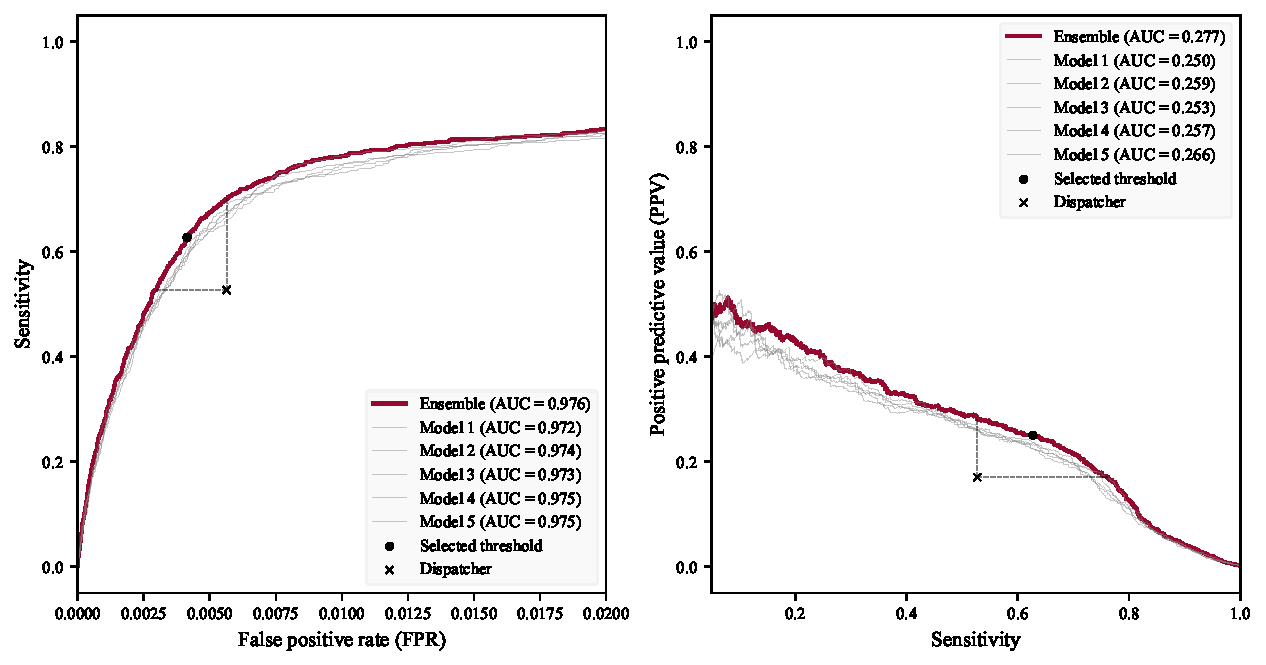
\includegraphics[width=0.9\textwidth]{paper_retrospective/figure1.pdf}
    \caption[Receiver operator characteristic (ROC) curve and PPV-sensitivity curve for stroke recognition.]{Receiver operator characteristic (ROC) curve and PPV-sensitivity curve. Left, the ROC curve and, right, PPV-sensitivity curve (precision-recall curve). Models 1-5 are the individual models that make up the ensemble model.}
    \label{fig_retrospective:figure1}
\end{figure}
% \todo[inline]{Insert Figure 1}

\begin{figure}[t]
    \centering
    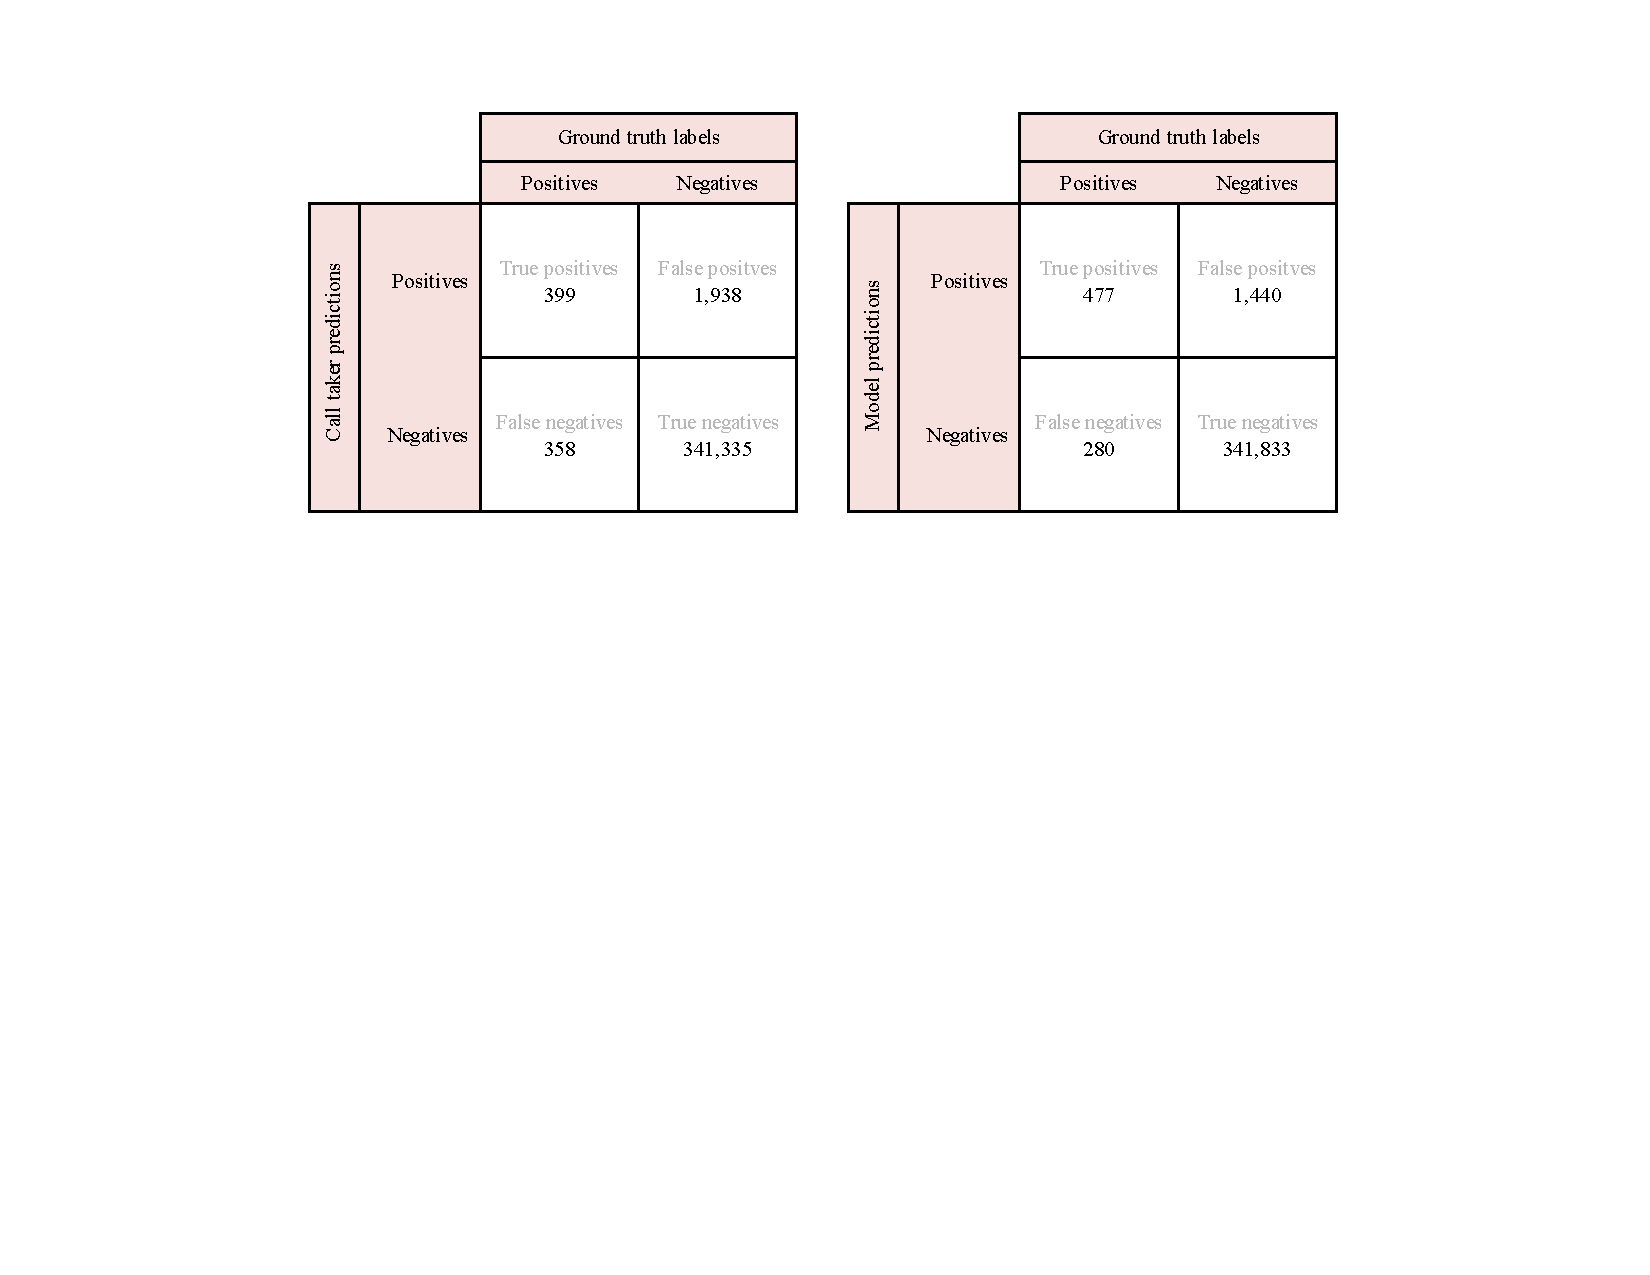
\includegraphics[width=0.9\textwidth]{paper_retrospective/figure2.pdf}
    \caption[Prediction confusion matrices for stroke recognition.]{Prediction confusion matrices. Confusion matrices of predictions for call takers and the model on the test set. Numbers for the model are given as the rounded mean over eleven runs.}
    \label{fig_retrospective:figure2}
\end{figure}
% \todo[inline]{Insert Figure 2}


\subsection{Model explainability}

Among the words with a positive rank score, several words are synonymous with stroke, such as ``blood clot", ``haemorrhagic stroke", and ``stroke". Ambulances are rarely dispatched because the MH-1813 is not intended for emergencies. Therefore, a word like ``ambulance" may also be a strong indicator of call-taker recognition, which the model has learned to mimic. Additionally, most of the remaining words can be linked to stroke-related symptoms such as ``double vision", ``difficulties speaking", and ``hangs". Particularly, words describing the side of the body where symptoms occur ranked high (such as ``left", ``right", and ``side"). Finally, some words were also related to the sudden onset of symptoms (including ``suddenly" and ``minutes").
% \todo[inline]{Insert Table 2}
\begin{table}[t]
    \centering
    \caption[Overall stroke recognition performance of model compared to call takers.]{Overall performance on MH-1813 test data, performance without 1-1-2 training data, and performance on data from 2021 without diagnostic categories as well as performance on MH-1813 based on demographic subgroups (age/sex) [mean (95\% CI)].}
    \label{tab_retrospective:table2}
    \resizebox*{0.98\textwidth}{!}{%
    \begin{tabular}{l|ccccc}
        \toprule
                    & F1-score [\%] $\uparrow$ & Sensitivity [\%] $\uparrow$ & PPV [\%] $\uparrow$ & \makecell{FOR [\%] $\downarrow$ \\ (1 - specificity)} & \makecell{FPR [\%] $\downarrow$ \\ (1 - NPV)} \\

        \midrule
        \multicolumn{6}{c}{\emph{Overall}} \\
        \midrule
        Call takers & 25.8 (23.7-27.9) & 52.7 (49.2-56.4) & 17.1 (15.5-18.6) & 0.105 (0.094-0.116) & 0.565 (0.539-0.590) \\
        Model       & 35.7 (35.0-36.4) & 63.0 (62.0-64.1) & 24.9 (24.3-25.5) & 0.082 (0.079-0.085) & 0.419 (0.413-0.426) \\

        \midrule
        \multicolumn{6}{c}{\emph{Without 112 training data}} \\
        \midrule
        Model       & 32.4 (31.8-33.1) & 60.4 (59.3-61.4) & 22.2 (21.6-22.7) & 0.088 (0.085-0.091) & 0.467 (0.460-0.474) \\

        \midrule
        \multicolumn{6}{c}{\emph{On MH-1813 data without diagnostic category}} \\
        \midrule
        Model       & 32.6 (31.9-33.4) & 48.3 (47.2-49.4) & 24.7 (23.9-25.3) & 0.153 (0.148-0.158) & 0.435 (0.427-0.443) \\

        \midrule
        \multicolumn{6}{c}{\emph{18-64 years}} \\
        \midrule
        Call takers & 15.9 (13.1-18.5) & 50.5 (43.6-57.2) & 9.40 (7.61-11.18) & 0.036 (0.028-0.043) & 0.353 (0.331-0.375) \\
        Model       & 22.9 (21.8-24.0) & 54.1 (52.1-56.3) & 14.5 (13.8-15.3) & 0.033 (0.031-0.035) & 0.231 (0.226-0.236) \\ 

        \midrule
        \multicolumn{6}{c}{\emph{65+ years}} \\
        \midrule
        Call takers & 32.9 (30.1-35.7) & 53.5 (49.4-57.6) & 23.7 (21.4-26.0) & 0.401 (0.352-0.449) & 1.467 (1.373-1.560) \\
        Model       & 42.8 (41.9-43.7) & 66.3 (65.1-67.5) & 31.6 (30.8-32.4) & 0.290 (0.278-0.303) & 1.224 (1.198-1.249) \\

        \midrule
        \multicolumn{6}{c}{\emph{Male}} \\
        \midrule
        Call takers & 30.2 (27.2-33.3) & 53.9 (49.1-58.9) & 21.0 (18.5-23.5) & 0.124 (0.105-0.141) & 0.542 (0.506-0.580) \\
        Model       & 39.0 (38.0-40.1) & 63.7 (62.3-65.2) & 28.1 (27.3-29.0) & 0.097 (0.093-0.102) & 0.435 (0.425-0.445) \\

        \midrule
        \multicolumn{6}{c}{\emph{Female}} \\
        \midrule
        Call takers & 21.9 (19.1-24.6) & 51.3 (46.0-56.6) & 13.9 (12.0-15.8) & 0.090 (0.076-0.103) & 0.582 (0.547-0.616) \\
        Model       & 32.4 (31.4-33.4) & 62.3 (60.7-63.8) & 21.9 (21.1-22.7) & 0.069 (0.066-0.073) & 0.407 (0.399-0.416) \\
        
        \bottomrule
    \end{tabular}%
    }
\end{table}


Among the words with a negative rank score, most were strong indicators for specific conditions, symptoms, or body parts that are unrelated to stroke (such as ``tetanus", ``pregnant", ``swollen", ``fever", and ``the knee"). Another group of words used to describe aspects of treatment that are unlikely to be addressed in a stroke call included ``prescription", ``bandage", and ``OTC". Finally, a small group of words described institutions that are not commonly involved in stroke treatment (such as ``psychiatric", ``the emergency room", and ``the police").


\section{Discussion}

Our results showed that a machine learning framework can substantially improve stroke recognition in medical helpline calls compared to solely relying on human call-takers. This improvement was observed across all performance metrics and for basic patient demographics (age and sex). Our occlusion analysis revealed that the model relied on the relevant predictive features associated with call-taker triaging, patient symptoms, and treatment.

This study does not imply that a machine learning model can replace medical call-takers. The effectiveness of the model is fully reliant on the conversation between the call-taker and caller and the call-taker's ability to skillfully triage the patient. Instead, the model should be used as a supportive tool for call-takers in the decision-making process, contributing to a higher recognition of patients with stroke and potentially boosting the confidence of call- takers in their decisions. A similar machine learning model designed to predict cardiac arrest was tested in a randomised controlled trial (RCT) at CEMS.15 The results highlighted the necessity of incorporating input from call-takers. The machine learning model for cardiac arrest has subsequently been implemented in daily practice at CEMS, in a setup similar to the one presented in our study. However, implementation of our framework requires further investigation. The relative performance gap between call-takers and the model was larger in our study than in the cardiac arrest study,15 which may affect the results of a potential RCT. To support future work and discussions beyond the scope of this study, \cref{app:retrospective} includes the results of a simulation of a live implementation where call-takers are assumed to follow a set of fixed rules based on the output of the machine learning framework.

The performance gap between the model and call-takers could be explained by the rarity of stroke calls to MH-1813 (0.250\% of all calls in 2021), which might affect call-taker awareness of stroke as a possible cause of certain symptoms. Additionally, certain stroke symptoms are so rare that some call-takers may never encounter them, increasing the risk of false negatives. The model was trained on more calls than any single call-taker would handle in a lifetime, enabling it to recognise even rare descriptors of stroke. The model is specifically trained to recognise strokes and exclusively learns from actual stroke descriptions, unlike call-takers, who are trained with generalised teaching materials to triage many different conditions. Therefore, call-takers may not have received specific training for patients with stroke and may never have encountered them.

The model performed significantly better on men than on women. This could be attributed to several factors. First, the model may have learned to mimic call-takers with the same bias. Second, women may experience different and challenging-to-identify symptoms than men \cite{cite29, cite30}. Third, a higher prevalence of male patients with stroke was observed in the training data. Despite these potential sources of bias, the model exhibited less bias than call-takers did. That is, the relative performance improvements were higher for women than for men. This bias could be further reduced using advanced data augmentation and balanced data when training a machine learning model. However, such measures may degrade overall performance.

This study has some limitations. First, the mapping of call recordings to electronic records was incomplete due to technical limitations in the CAD registry, which limited the number of calls available to us. Of note, there was no obvious pattern of bias related to the unmapped calls, and we included all calls with matching audio files, regardless of dispatcher performance. The results could potentially be improved if more calls were available for analysis. Second, calls without a call-taker indicated diagnostic category were not included in the validation and test data because the call-taker's performance could not be evaluated. Moreover, in exploratory analyses, the model performed worse on these calls, which might be attributed to differences in population characteristics (\cref{tab_retrospective:table3}). Finally, the ground truth stroke labelling relied on the patient-reported time of onset being exact; however, estimating the accuracy of the timestamps in DanStroke was impossible.

The proposed machine learning framework can be improved. In preliminary experiments, we tested convolutional, recurrent, and self-attention architectures for text classification; however, this did not improve the model. One promising path is to leverage the abundance of non-stroke calls. Self-supervised learning techniques for speech and text data can be used to improve speech recognition and text classification models. This approach can enable direct classification from audio input without speech recognition. Finally, incorporating additional data from CAD records through multitask learning could be used to inform the classifier and predict the diagnostic category to improve its ability to identify more fine-grained characteristics of non-stroke calls.

In conclusion, using the largest collection of audio calls from patients with stroke to date, we developed a machine learning framework that significantly outperformed human call-takers in stroke recognition in medical helpline calls. The framework can assist human call-takers during medical helpline calls. Ideally, this would enable a higher recognition of patients with stroke in the prehospital setting, benefiting both patient outcomes and health service resource allocation.

\subsection{Contributors}

JW, JDH and LB share lead authorship and contributed equally to the original drafting of the paper, review and editing, data curation, formal analysis, methodology, validation, and conceptualisation. JDH and LB contributed to software development and funding acquisition. SNFB contributed to the conceptualisation, data curation, funding acquisition, supervision, and writing - review and editing. LM contributed to conceptualisation, funding acquisition, project administration, supervision, and writing - review and editing. MS contributed to supervision and writing - review and editing. HC contributed to the methodology, supervision, and writing - review and editing. CK contributed to the conceptualisation, funding acquisition, methodology, project administration, supervision, and writing - review and editing. HCC contributed to the conceptualisation, data curation, funding acquisition, methodology, project administration, supervision, and writing - review and editing. HCC and CK share last authorship. The three lead authors directly accessed and verified the underlying data reported in this manuscript. JW's affiliations are exclusively academic.


\section{Methods}

\subsection{Study design}

We used call recordings and registry data from the Copenhagen Emergency Medical Services (CEMS) and the Danish Stroke Registry \cite{cite16} from 2015 to 2020. These data were used to train a machine learning model to classify medical helpline calls as stroke or non-stroke. We compared the performances of the model with that of the call-taker using data from 2021.

\subsection{Data sources}

\subsubsection{CEMS}

The CEMS is responsible for providing prehospital telehealth services in the Capital Region of Denmark, with a catchment area of 1.9 million \cite{cite17}. CEMS operates two call lines: the 1-1-2 emergency line, similar to 9-1-1 in the United States, intended for acute conditions. The other is the medical helpline 1813 (MH-1813, pronounced ``'eighteen-thirteen") intended for non- life-threatening conditions that cannot wait until a general practitioner is available.18

Call-takers for both lines, who are nurses, paramedics, or physicians, can dispatch ambulances. The condition suspected by the call-taker is categorised based on a predefined diagnostic index and stored in an electronic record using a computer-aided dispatch (CAD) system. The CAD records are associated with the Danish civil registration number (CPR number) \cite{cite19} of the patient. The CPR number is a unique identification assigned to all Danish residents. It is used for interactions with health services and registries, enabling cross- referencing of the data sources used in this study. The call audio is recorded and stored separately from the CAD recordings using a telephone system.

\subsubsection{Danish Stroke Registry (DanStroke)}

All patients with stroke admitted to a Danish hospital within 5 days of symptom onset are recorded in the Danish Stroke Registry \cite{cite16}, also known as DanStroke. This record includes the patient-reported time of onset, stroke type (haemorrhagic, ischaemic, or transitory ischaemic attack), and CPR number of the patient.

\subsubsection{Data ethics}

The Danish Data Protection Agency (P-2021-475) approved this study. Danish law did not require approval from the Scientific Ethics Committee because the data were registry-based. CEMS approved the transcription of all calls made to 1-1-2 and MH-1813. All electronic records were anonymised before analysis, and the researchers did not inspect the calls manually.

\subsection{Study scope}

Stroke prevalence in calls made to the MH-1813 is lower than that in calls made to 1-1-2. Patients with stroke may exhibit different symptoms and symptom severity because MH- 1813 is meant for low-acuity incidents, leading to reduced recognition. In addition, MH-1813 call-takers dispatch high-priority transport less frequently, which may affect optimal treatment timing. Therefore, we focused on MH-1813 in this study.

\subsection{Stroke dataset}

\subsubsection{Cross-referencing data sources}

From the CAD medical records, we included all calls that could be matched to a corresponding audio file. for 1-1-2 and MH-1813 from 2015 to 2021 for patients older than 18. The CAD records were matched with the telephone call recordings based on the call start, call duration, and call-taker identity. Due to data incompleteness, and the way the audio data is stored, at CEMS, 2,730,199 contacts could not be matched to their corresponding audiofile, however, 2,361,178 contacts were successfully matched. We found no obvious pattern in the matched and unmatched calls and we included all calls with at matching audio file. Next, a call was regarded as a case of ground truth stroke positive when the CPR number in the CAD record matched that of a DanStroke record, and the patient-reported time of onset was close to the call start time. We allowed a window of 72 hours before and 24 hours after the call starts to account for uncertainty in recording stroke onset time. We excluded calls involving subarachnoid haemorrhage cases. Finally, we considered a call to be a call-taker stroke positive when the call-taker selected the stroke diagnostic category during the call and dispatched an ambulance with the appropriate level of response \cite{cite20}. To ensure that the effect of the machine learning framework was not overestimated, we excluded calls where diagnostic category had not been registered from the final testing. We still reported the population characteristics and model performance of this group of calls to assess potential bias introduced by excluding them. A data-flow diagram is included in \cref{app:retrospective}. The resulting dataset is the largest dataset of audio files from stroke calls collected to date.

\subsubsection{Dataset splitting}

We reserved all the MH-1813 calls from 2021 for testing. We used stratified sampling to split the MH-1813 calls from 2015 to 2020 into six folds: one for validation and five for training. The calls were stratified based on the ground truth stroke label and the presence of a diagnostic category. Only calls without diagnostic categories were included in the training set. The 1-1-2 calls were used only for training; however, calls from 2021 were discarded to avoid temporal overlap with the test period.

As expected, the 1-1-2 training data differed from the MH-1813 data regarding age, male/female ratio, and stroke prevalence (\cref{tab_retrospective:table3}). We performed an ablation study where 1- 1-2 data were not used for training to assess whether this difference negatively impacted model performance. The training, validation, and test subsets of the MH-1813 data had similar characteristics, whereas the 2021 data without diagnostic categories differed in age and sex.

\subsection{Machine learning pipeline}

We employed a two-step machine learning pipeline. First, a call was transcribed using the speech recognition model. Second, the transcript was used as input for the text classification model. The final output score was used to classify whether the call concerned a stroke. The pipeline is illustrated in \cref{app:retrospective}.

% \todo[inline]{Insert Table 3}
\begin{table}[t]
    \centering
    \caption[Words with the largest positive and negative ranking score in calls predicted as stroke and non-stroke, respectively.]{English translation of words with the largest positive and negative ranking score in calls predicted as stroke and non-stroke, respectively.}
    \label{tab_retrospective:table3}
    \resizebox*{0.98\textwidth}{!}{%
    \begin{tabular}{l|lr|lr}
        \toprule
                    & \multicolumn{2}{c|}{Positive ranking score} & \multicolumn{2}{c}{Negative ranking score} \\
        \midrule
                    & \multicolumn{2}{c|}{Stroke predictions, $D=1,897$} & \multicolumn{2}{c}{Non-stroke predictions, $D=342,133$} \\
        \midrule
                    & Word, $w$ \textit{(translated)} & Occurences, $D^{(w)}$ & Word, $w$ \textit{(translated)} & Occurences, $D^{(w)}$ \\
        \midrule
        1.  & Ambulance & 1,680 & Tetanus & 4,378 \\        
        2.  & Blood clot & 895 & Pregnant & 8,749 \\        
        3.  & Left & 1,108 & Cut & 7,592 \\        
        4.  & Right & 1,050 & Bandage & 4,561 \\        
        5.  & Double vision & 84 & Amager (a location) & 23,776 \\        
        6.  & The words & 344 & O'clock & 94,436 \\        
        7.  & Suddenly & 783 & The emergency room & 42,809 \\        
        8.  & Arm & 709 & The police & 2,903 \\        
        9.  & Side & 1,139 & Swollen & 60,559 \\        
        10. & Stroke & 117 & Over the counter (OTC) & 4,641 \\        
        11. & Double & 113 & The neck & 30,151 \\        
        12. & Control & 134 & Fever & 112,586 \\        
        13. & Call & 39 & Prescription & 5,450 \\        
        14. & Numb & 94 & Centimetre & 12,026 \\        
        15. & Minutes & 763 & The knee & 8,875 \\        
        16. & Difficulties speaking & 44 & The pharmacy & 10,085 \\        
        17. & Haemorrhagic stroke & 133 & The stomach & 42,105 \\        
        18. & Hand & 297 & Psychiatric & 3,688 \\        
        19. & The ambulance & 521 & Pneumonia & 7,597 \\        
        20. & Slurred speech & 58 & Stomach pain & 10,551 \\        
        21. & Blood clots & 224 & Stool & 19,155 \\        
        22. & Fast & 663 & The ribs & 3,928 \\        
        23. & Express & 44 & Bleed & 10,501 \\        
        24. & Blood thinner & 259 & Bleeding & 24,313 \\        
        25. & Incoherent & 15 & Ribs & 2,941 \\        
        26. & Lopsided & 211 & Broken & 19,415 \\        
        27. & Reduced & 528 & Inflammation & 10,050 \\        
        28. & Hangs & 628 & Common cold & 8,127 \\        
        29. & Transient & 48 & Morning or morrow & 78,558 \\        
        30. & Not making sense & 14 & Swelling & 17,762 \\        
        \bottomrule
    \end{tabular}%
    }
\end{table}


\subsubsection{Speech recognition}

The call recordings from the CEMS were stored as 8-bit linear pulse-code modulated audio, sampled at 8 kHz. A call was converted into a log-Mel spectrogram before being input into the speech recognition model. This conversion is a commonly used input representation for speech-processing tasks, which facilitates the identification of linguistic content in audio signals. We used a speech recognition model with a neural network architecture \cite{borgholt_endtoend_2020}, consisting of two-dimensional convolutional layers \cite{cite22} and blocks of bidirectional long short-term memory layers \cite{hochreiter_long_1997} The output is a sequence of probability distributions over characters of the Danish alphabet, which were then converted into a human-readable transcript using a greedy decoder \cite{graves_connectionist_2006}.

\subsubsection{Text classification}

As input for the classification model, each transcript was transformed into a fixed-size bag- of-words vector, which encoded the occurrence of word and character ($n$-grams) in a fixed vocabulary. The feature selection procedure is detailed in \cref{app:retrospective}. The model was constructed as an ensemble \cite{hansen_neural_1990} of five identical, independently trained models. Each consists of a stack of neural network layers commonly referred to as a multi-layer perceptron \cite{rosenblatt_perceptron_1958}. The final layer has a single scalar output and applies a sigmoid nonlinearity to produce an output score between zero and one.

\subsubsection{Threshold calibration and ensembling}

We selected the prediction threshold as the harmonic mean of the thresholds for each model in the ensemble to ensure that the sensitivity and positive predictive value (PPV) were equal to those of the call-takers. This simplifies the comparison by ensuring a trade-off between sensitivity and PPV, similar to that of call-takers.

As the threshold differed for each model in the ensemble, computing the ensemble output score as the average output score of the individual models would not be meaningful. Instead, we first subtracted the threshold from the output score in the logit space (before sigmoid nonlinearity) for each model to obtain the same threshold (0.5). Subsequently, we defined the ensemble output score as the average of the centred output scores. The exact equations are provided in \cref{app:retrospective}.

\subsubsection{Model training}

The speech recognition model was trained on 3,811 manually transcribed random calls (173 h) from the CEMS as part of a previous project.14 These calls exclusively originated from 1- 1-2 between 2015 and 2018, ensuring no overlap with the test data used for the text classification model. The model was trained using a connectionist temporal classification objective \cite{graves_connectionist_2006}.

We trained five models for the text classification ensemble using binary cross-entropy after transcribing all calls in the dataset using the speech recognition model. One training fold was used for early stopping, whereas the remaining four folds and 1-1-2 data were used for training. Thus, each model in the ensemble was trained and validated using different datasets. We ran a grid search with 96 different hyperparameter configurations and selected the ensemble model with the best F1 score for the validation set.

\subsection{Model explainability}\label{sec_retrospective:model_explainability}

We performed an \emph{occlusion analysis} to better understand the predictions of the text classification model. This involved removing all instances of a given word from the input transcript to evaluate its impact on the model output. The word was removed before vectorisation, such that all word and character $n$-grams associated with the word were discarded. Specifically, let $z^{(n, d, w)}$ be the logit output of model $n$ in the ensemble for transcript $d$ when the word $w$ is occluded. For transcript $d$, we computed the word impact score $i^{(d, w)}$ as the mean difference between the logit before and after occlusion.
%
\begin{equation}
    i^{(d,w)} = \frac{1}{N_d} \sum_{n=1}^{N_d} \left( z^{(n, d)} - z^{(n, d, w)} \right) \enspace .
\end{equation}
%
We used the logit output to compute the impact score because the difference in sigmoid-normalised output is biased towards zero for values close to 0 or 1. To select words for inspection, we computed a ranking score, $r^{(w)}$, as the sum of the signed squares of the impact:
%
\begin{equation}
    r^{(w)} = \sum_{d=1}^{N} \text{sign}\left( i^{(d, w)} \right) \left( i^{(d,w)}\right) ^2 \enspace .
\end{equation}
%
where $\text{sign}$ represents the sign function. Squaring $i^{(d,w)}$ favours rare features with a high impact over common features with a low impact.

\subsection{Statistical analysis}

We report the F1-score, sensitivity, PPV, false omission rate (FOR, equal to 1- negative predictive value), and false positive rate (FPR, equal to 1 - specificity). Due to the imbalanced nature of the dataset, the negative predictive value and specificity were greater than 99\% for all cases. We reported FOR and FPR instead because such large numerical values exhibit low relative variance, thereby obfuscating comparisons. Finally, we report the prediction confusion matrices, receiver operator characteristic (ROC) curve, and PPV- sensitivity curve, commonly known as the precision-recall curve. All results are reported with up to three significant digits.

We present the results with and without 1-1-2 training data, subgroup analyses based on age (18-64/65+) and sex (male/female), and call-takers performance. We also report the model performance on calls without a diagnostic category from the test year 2021 to assess potential data bias. We tested our results for statistical significance using approximate permutation tests, paired or independent, as appropriate and computed 95\% confidence intervals (CIs) using bootstrapping \cite{dwass_modified_1957,eden_validity_1933}. In our assessment, we accounted for random variation associated with model training by basing the means, tests, and CIs on the predictions of 11 randomly initialised training runs. Statistical significance was defined as a two-sided p-value of < 0.05.

We used the model with the median F1-score out of the 11 runs for the occlusion analysis. We listed the 30 words with the highest positive ranking scores for calls classified as stroke and the 30 words with the highest negative ranking scores for calls classified as non-stroke.

\subsection{Role of the funding source}

The grant providers had no role in the study design, data collection, analysis, interpretation, manuscript writing, or publication decision. Corti provided additional funds and technical expertise to develop the models. Corti was not financially compensated for this, and the project was part of its research initiatives, which were conducted in cooperation with several universities and the Innovation Fund Denmark. Corti owns the rights to the models and source code.


\section{Data availability}

The datasets used to evaluate call-taker performance and to train and evaluate the machine learning framework are legally restricted by Danish patient privacy and secrecy laws and are therefore, not publicly available. The data can be made available from the publication date but requires a Data Access Agreement, which is examined and approved by the ethics committees that approved this research. For the same reason, the machine learning framework trained in this study is not publicly available; however, instructions on how to train it are included in the main manuscript and supplementary material. The source code can be shared using a Creative Commons NC-ND 4.0, an international licence, upon reasonable written request to the corresponding author, and requires a data use agreement.


\section{Declaration of interests}

JDH and LB received funding from the Innovation Fund Denmark. JDH and LB used Corti and hold stock warrants. LM is a co-founder, stockholder, and the Chief Technology Officer of Corti. JW received funding from Trygfonden. SNFB has no conflicts of interest to declare. HC has received funding from the Velux Foundation, Tværsfonden, Helsefonden, Hartmann Fonden, Lundbeck Foundation, and Novo Nordisk Foundation; royalties from Gyldendal; honoraria from Bayer and Bristol Meyers Squibb, and is chair of Action Plan for stroke in Europe Implementation, Co-chair of the Scientific Stroke Panel EAN and Senior Guest Editor of AHA Stroke. MS has no conflicts of interest to declare. HCC has no conflicts of interest to declare. CK received funding from the Novo Nordisk Foundation and is the chair of the Danish Resuscitation Council and vice chair of the Danish Stroke Society. Both positions are unpaid.


\section*{Acknowledgements}

We thank the staff of the CEMS for their role in generating the data used in this study. We thank Emilie Grunddal Pedersen, Mette Bjerg Lindhøj, and Jens Morten Haugård for their help and cooperation in accessing the data sources. We also thank the Centre for IT and Medical Technology (CIMT) and Corti employees Akihiro Inui and Nathaniel Joselson for their assistance in setting up and using the cloud-computing environment for training and evaluating the machine learning framework of this study.

}
